\chapter{Kümeler ve Küme Üzerine Muhakeme}
\label{chap:kumeler}


\par\smallskip{\sffamily\bfseries\color{cAcc}Öğrenme Hedefleri}\nopagebreak

\begin{itemize}\setlength{\itemsep}{2pt}\setlength{\parskip}{0pt}
\item Küme, alt küme ve temel küme işlemlerini biçimsel olarak tanımlayabilme.
\item Küme eşitliğini çift kapsama yöntemiyle ispatlayabilme.
\item Kümeler için De Morgan yasalarını ispatlayabilme.
\end{itemize}

\section*{Bölüme Genel Bakış: Kümeler ve Matematiğin Dili}

Küme kavramı modern matematiğin ortak dilidir; ama bu dil tarihsel olarak geç ve sancılı doğdu. Georg Cantor 1870’lerde sonsuz kümeleri karşılaştırmaya giriştiğinde, ‘bir araya getirilmiş nesneler topluluğu’ fikrini matematiğin merkezine taşıdı. Gottlob Frege bu fikri mantığın temeli yapmayı denedi; ancak Bertrand Russell’ın 1901’de bulduğu paradoks, ‘her özellik bir küme tanımlar’ sezgisinin tutarsız olduğunu gösterdi. Ernst Zermelo’nun 1908’deki aksiyomları ve sonraki Fraenkel katkıları küme kavramını sağlam bir temele oturttu.

Bu bölüm kümeleri sezgisel düzeyde tanıtır, ama biçimsel muhakemeyi — özellikle çift kapsama tekniğini — merkeze alır. Amaç yalnızca küme işlemlerini öğretmek değil; ‘iki kümenin eşit olduğunu nasıl ispatlarız?’ ve ‘en sezgisel görünen ilke neden paradoksa yol açabilir?’ gibi soruları çalışarak öğrenciyi matematiksel titizliğe alıştırmaktır. Küme dili sağlam kurulduğunda, sonraki bütün bölümler (bağıntılar, fonksiyonlar, kardinalite) onun üzerine inşa edilir.

\section{Temel Tanımlar}

\begin{tcolorbox}[bookbox,colback=cDef]\textbf{\textsf{\textcolor{cAcc}{Tanım.}}}\quad Bir A kümesi için x ∈ A, “x, A’nın elemanıdır” demektir. A ⊆ B (A, B’nin alt kümesidir), her x için x ∈ A ⇒ x ∈ B koşuluyla tanımlanır. A = B ancak ve ancak A ⊆ B ve B ⊆ A.\end{tcolorbox}

Boş küme ∅ hiçbir elemanı olmayan kümedir ve her kümenin alt kümesidir. Bir A kümesinin tüm alt kümelerinin kümesine kuvvet kümesi denir ve P(A) ile gösterilir.

\section{Küme İşlemleri}

Birleşim A ∪ B = \{x: x ∈ A ∨ x ∈ B\}; kesişim A ∩ B = \{x: x ∈ A ∧ x ∈ B\}; fark A \textbackslash{} B = \{x: x ∈ A ∧ x ∉ B\}. Evrensel küme U içinde tümleyen Aᶜ = U \textbackslash{} A. Kartezyen çarpım A × B = \{(a, b): a ∈ A, b ∈ B\}.

\begin{figure}[htbp]
\centering
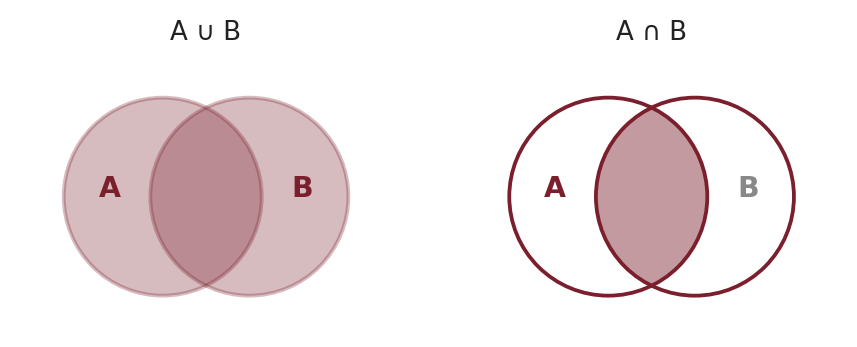
\includegraphics[width=0.85\linewidth]{figs/venn.png}
\caption{Birleşim (A ∪ B) ve kesişim (A ∩ B).}
\end{figure}

\section{Küme Üzerinde İspat: Çift Kapsama}

İki kümenin eşitliğini göstermenin standart yolu her iki kapsamayı ayrı ayrı ispatlamaktır. Bu, küme muhakemesinin temel tekniğidir.

\begin{tcolorbox}[bookbox,colback=cEx]\textbf{\textsf{\textcolor{cAcc}{Örnek.}}}\quad İddia: (A ∪ B)ᶜ = Aᶜ ∩ Bᶜ (De Morgan).\par\medskip{}İspat: x ∈ (A ∪ B)ᶜ ⇔ x ∉ A ∪ B ⇔ ¬(x ∈ A ∨ x ∈ B) ⇔ (x ∉ A) ∧ (x ∉ B) ⇔ x ∈ Aᶜ ∧ x ∈ Bᶜ ⇔ x ∈ Aᶜ ∩ Bᶜ. Her adım bir mantıksal eşdeğerlik olduğundan iki küme aynı elemanlara sahiptir. ∎\end{tcolorbox}

\begin{tcolorbox}[bookbox,colback=cEx]\textbf{\textsf{\textcolor{cAcc}{Örnek.}}}\quad İddia: A ⊆ B ise P(A) ⊆ P(B).\par\medskip{}İspat: X ∈ P(A) olsun, yani X ⊆ A. A ⊆ B olduğundan geçişlilikle X ⊆ B, dolayısıyla X ∈ P(B). Keyfi X için gösterildiğinden P(A) ⊆ P(B). ∎\end{tcolorbox}

\begin{tcolorbox}[bookbox,colback=cDep]\textbf{\textsf{\textcolor{cAcc}{Muhakeme/Felsefe Derinleştirmesi — Naif küme kuramının sınırı: Russell paradoksu}}}\quad “Her özellik bir küme tanımlar” (sınırsız kapsam belirleme) ilkesi çekicidir ama tutarsızdır. R = \{x: x ∉ x\} kümesini düşünün: R ∈ R ise tanımı gereği R ∉ R; R ∉ R ise yine tanımı gereği R ∈ R. Her iki durumda çelişki. Russell’ın 1901’de bulduğu bu paradoks, küme kavramının aksiyomlarla (ZFC) sınırlandırılması gerektiğini gösterdi. Öğrenci için ders şudur: en sezgisel görünen ilke bile denetlenmeden kabul edilemez — bu, dersin ‘aksiyomatik dikkat’ temasının çekirdeğidir.\end{tcolorbox}

\section{İleri Örnekler: Küme Özdeşliklerinin İspatı}

Aşağıdaki örnekler çift kapsama ve eşdeğerlik-zinciri tekniklerini pekiştirir. Her adımda küme işleminin karşılık geldiği mantıksal bağlacı (∩ ↔ ∧, ∪ ↔ ∨, tümleyen ↔ ¬) izlemek, ispatı neredeyse mekanik hâle getirir.

\begin{tcolorbox}[bookbox,colback=cEx]\textbf{\textsf{\textcolor{cAcc}{Örnek.}}}\quad Dağılma yasası: A ∩ (B ∪ C) = (A ∩ B) ∪ (A ∩ C).\par\medskip{}İspat: x ∈ A ∩ (B ∪ C) ⇔ x ∈ A ∧ (x ∈ B ∨ x ∈ C) ⇔ (x ∈ A ∧ x ∈ B) ∨ (x ∈ A ∧ x ∈ C) ⇔ x ∈ (A ∩ B) ∪ (A ∩ C). Ortadaki adım, ‘ve’nin ‘veya’ üzerine dağılmasıdır; küme özdeşliği doğrudan mantıksal dağılmadan gelir. ∎\end{tcolorbox}

\begin{tcolorbox}[bookbox,colback=cEx]\textbf{\textsf{\textcolor{cAcc}{Örnek.}}}\quad Farkın dağılması: A \textbackslash{} (B ∪ C) = (A \textbackslash{} B) ∩ (A \textbackslash{} C).\par\medskip{}İspat: x ∈ A \textbackslash{} (B ∪ C) ⇔ x ∈ A ∧ ¬(x ∈ B ∨ x ∈ C) ⇔ x ∈ A ∧ x ∉ B ∧ x ∉ C ⇔ (x ∈ A ∧ x ∉ B) ∧ (x ∈ A ∧ x ∉ C) ⇔ x ∈ (A \textbackslash{} B) ∩ (A \textbackslash{} C). ∎\end{tcolorbox}

\begin{tcolorbox}[bookbox,colback=cEx]\textbf{\textsf{\textcolor{cAcc}{Örnek.}}}\quad Kesişim ve kuvvet kümesi: P(A ∩ B) = P(A) ∩ P(B).\par\medskip{}İspat: X ∈ P(A ∩ B) ⇔ X ⊆ A ∩ B ⇔ (X ⊆ A) ∧ (X ⊆ B) ⇔ X ∈ P(A) ∧ X ∈ P(B) ⇔ X ∈ P(A) ∩ P(B). Buna karşılık P(A ∪ B) = P(A) ∪ P(B) genelde YANLIŞTIR: A = \{1\}, B = \{2\} için \{1,2\} ∈ P(A ∪ B) iken P(A) ∪ P(B)’de değildir. ∎\end{tcolorbox}

\begin{tcolorbox}[bookbox,colback=cEx]\textbf{\textsf{\textcolor{cAcc}{Örnek.}}}\quad Sonlu sayma (içerme–dışarma): |A ∪ B| = |A| + |B| − |A ∩ B|.\par\medskip{}Gözlem: A ∪ B’yi ayrık parçalara ayırırsak (yalnız A, yalnız B, ortak) her elemanı tam bir kez sayarız; |A| + |B| toplamı ortak elemanları iki kez saydığından bir kez geri çıkarılır. Bu ilke olasılık ve kombinatorikte sürekli kullanılır.\end{tcolorbox}

\begin{tcolorbox}[bookbox,colback=cMis]\textbf{\textsf{\textcolor{cAcc}{Yaygın Kavram Yanılgıları}}}\quad \textbf{“∈ ile ⊆ aynı şeydir.” — }‘∈’ eleman olmayı, ‘⊆’ alt küme olmayı belirtir. 1 ∈ \{1,2\} doğrudur ama 1 ⊆ \{1,2\} anlamsızdır; \{1\} ⊆ \{1,2\} doğrudur.\par\medskip{}\textbf{“∅ ile \{∅\} aynıdır.” — }∅ elemanı olmayan kümedir; \{∅\} ise bir elemanı (boş kümeyi) olan kümedir. Dolayısıyla |\{∅\}| = 1.\par\medskip{}\textbf{“A ⊆ B ise A ∈ B’dir.” — }Alt küme olmak eleman olmayı gerektirmez. \{1\} ⊆ \{1,2\} doğrudur ama \{1\} ∈ \{1,2\} yanlıştır.\par\medskip{}\textbf{“P(A ∪ B) = P(A) ∪ P(B).” — }Genelde yanlıştır; kuvvet kümesi kesişimle uyumludur, birleşimle değil (yukarıdaki örnek).\par\medskip{}\textbf{“Kümenin elemanları sıralı ve tekrarlıdır.” — }Küme sıralamaya ve tekrara duyarsızdır: \{1,2,2,3\} = \{3,1,2\}. Sıra ve tekrar için diziler/çokküme kullanılır.\end{tcolorbox}

\section{Uygulama ve Eğitime Yansıma}

Küme dili, modern matematiğin ortak dilidir: fonksiyon, bağıntı, olasılık, topoloji ve cebir bu dille tanımlanır. Bu yüzden küme kavramını sağlam kurmak, sonraki her bölümün ön koşuludur. Eğitim açısından Venn şemaları, öğrenciyi görsel düzeyden (van Hiele 1) işlemleri çözümlemeye (2. düzey) taşıyan doğal bir köprüdür; ancak öğretmen, şemanın bir ispat değil bir sezgi aracı olduğunu vurgulamalı ve öğrenciyi çift kapsama gibi biçimsel gerekçeye yönlendirmelidir.

Ayrıca küme işlemleri, bilgisayar biliminde (veri tabanı sorguları, arama kümeleri) ve olasılıkta (olayların birleşimi/kesişimi) doğrudan kullanılır. Öğrenciye bu bağlantıları göstermek, soyut küme cebrini somut bir amaca bağlar ve motivasyonu güçlendirir.

\section{Yüksek Lisans Derinleştirmesi: Aksiyomatik Küme Kuramına Giriş}

Russell paradoksu, ‘her özellik bir küme tanımlar’ ilkesinin terk edilmesini zorunlu kıldı. Bunun yerine modern matematik, Zermelo–Fraenkel aksiyomlarını (seçim aksiyomuyla birlikte ZFC) benimser. Bu aksiyomlar hangi kümelerin var olduğunu denetimli biçimde belirler: genişleme (kümeler elemanlarıyla belirlenir), eşleme, birleşim, kuvvet kümesi, ayırma (bir kümenin bir özelliği sağlayan alt kümesi vardır — ama ‘her özellik’ bir küme vermez), sonsuzluk, düzenlilik ve seçim. ‘Ayırma’ aksiyomu, paradoksu tam da sınırsız kapsamı yasaklayarak engeller.

Bu çerçevede ‘tüm kümelerin kümesi’ gibi nesneler küme değil, ‘gerçek sınıf’ (proper class) olarak adlandırılır; bunlar başka kümelere eleman olamaz ve paradoks üretmezler. Küme–sınıf ayrımı, sezgisel ‘topluluk’ kavramının neden dikkatle sınırlandırılması gerektiğinin biçimsel karşılığıdır.

Çarpıcı olan, tüm matematiğin bu kümeler üzerine kodlanabilmesidir. Doğal sayılar bile kümelerle inşa edilir (von Neumann): 0 = ∅, 1 = \{∅\}, 2 = \{∅, \{∅\}\} ve genel olarak n + 1 = n ∪ \{n\}. Böylece her n, kendisinden küçük tüm doğal sayıların kümesidir ve |n| = n olur. Sıralı ikili (a, b) = \{\{a\}, \{a, b\}\} tanımıyla fonksiyonlar da kümeye indirgenir. Bu, kümeler kuramının neden matematiğin ‘temeli’ sayıldığını gösterir: en soyut yapılar bile, denetimli birkaç aksiyomdan doğan kümelerle ifade edilebilir.

\section{Simetrik Fark ve İndeksli İşlemler}

İki kümenin simetrik farkı A △ B = (A \textbackslash{} B) ∪ (B \textbackslash{} A), yani ‘tam olarak birinde bulunan’ elemanlardır. Simetrik fark değişmeli ve birleşmelidir; boş küme onun etkisiz elemanıdır (A △ ∅ = A) ve her küme kendisinin tersidir (A △ A = ∅). Bu özellikler, bir U kümesinin alt kümelerinin simetrik fark altında bir grup oluşturmasını sağlar — küme cebrinin cebirsel yapıya açıldığı ilk noktalardan biri.

\begin{tcolorbox}[bookbox,colback=cEx]\textbf{\textsf{\textcolor{cAcc}{Örnek.}}}\quad \textbf{Simetrik fark. }A = \{1, 2, 3\}, B = \{3, 4, 5\} için A \textbackslash{} B = \{1, 2\}, B \textbackslash{} A = \{4, 5\}, dolayısıyla A △ B = \{1, 2, 4, 5\}. Ortak eleman 3 dışarıda kalır; simetrik fark tam olarak ‘ortak olmayanları’ toplar.\end{tcolorbox}

İşlemler ikiden çok kümeye de genişler. Bir I indeks kümesi ve her i ∈ I için bir Aᵢ kümesi verildiğinde, birleşim ∪\_\{i∈I\} Aᵢ ‘en az bir Aᵢ’de bulunan’, kesişim ∩\_\{i∈I\} Aᵢ ise ‘tüm Aᵢ’lerde bulunan’ elemanlardır. Bu gösterim sonsuz sayıda kümeyle çalışmayı olanaklı kılar ve analiz ile topolojinin temel dilidir.

\begin{tcolorbox}[bookbox,colback=cEx]\textbf{\textsf{\textcolor{cAcc}{Örnek.}}}\quad \textbf{İndeksli kesişim. }Her n ∈ ℕ⁺ için Aₙ = (−1/n, 1/n) açık aralığı alınırsa ∩\_\{n\} Aₙ = \{0\}: her aralıkta bulunan tek nokta sıfırdır. Sonsuz bir kesişim tek bir noktaya ‘sıkışabilir’ — bu, limit fikrinin küme diliyle önizlemesidir.\end{tcolorbox}

Genelleştirilmiş De Morgan yasaları da geçerlidir: (∪\_\{i\} Aᵢ)ᶜ = ∩\_\{i\} Aᵢᶜ ve (∩\_\{i\} Aᵢ)ᶜ = ∪\_\{i\} Aᵢᶜ. Bu eşitlikler, sonlu durumdaki mantıksal çekirdeğin küme diline çevrilmiş hâlidir ve niceleyici olumsuzlama (Bölüm~\ref{chap:niceleyiciler}) ile — ¬(∃x) ⇔ ∀x¬ ve ¬(∀x) ⇔ ∃x¬ — doğrudan koşuttur. Böylece küme cebri ile yüklem mantığı arasındaki bağ görünür hâle gelir.

\section{Sıralı İkili ve Bağıntılara Köprü}

Kümeler yalnızca elemanları toplamakla kalmaz; başka yapıları da kodlar. Sıralı ikili (a, b), Kuratowski’nin tanımıyla \{\{a\}, \{a, b\}\} kümesidir; bu tanım (a, b) = (c, d) ⇔ a = c ∧ b = d özelliğini sağlar. Sıralı ikili sayesinde kartezyen çarpım, dolayısıyla bağıntı ve fonksiyon kavramları (Bölüm~\ref{chap:bagintilar} ve 12) tümüyle küme diline indirgenir.

Bu, kümelerin neden matematiğin ‘temeli’ sayıldığını bir kez daha gösterir: en dinamik görünen kavramlar — bir girdiyi çıktıya götüren fonksiyonlar, nesneler arası ilişkiler — bile statik kümelerle inşa edilebilir. Öğrenci için buradaki ders, soyutlamanın gücüdür: az sayıda ilkel kavram (eleman, küme, ∈) ve denetimli birkaç işlem, matematiğin tümünü taşıyacak kadar zengin bir dil kurar. Bu bölümde öğrenilen çift kapsama tekniği ise, bu dilde ‘kanıt’ yürütmenin en temel aracıdır ve sonraki her bölümde tekrar tekrar kullanılacaktır.

\section{Daha Fazla İspat ve Kanıt Stratejisi Seçimi}

Küme özdeşliklerini kanıtlamanın iki temel yolu vardır: eleman-temelli çift kapsama ve daha önce kanıtlanmış özdeşliklerden cebirsel türetme. Deneyimli bir kanıtlayıcı, probleme göre bu iki strateji arasında geçiş yapar. Aşağıdaki örnekler her iki yolu da gösterir.

\begin{tcolorbox}[bookbox,colback=cEx]\textbf{\textsf{\textcolor{cAcc}{Örnek.}}}\quad Kapsama ile eşitlik: A ⊆ B ⇔ A ∪ B = B.\par\medskip{}İspat (⇒): A ⊆ B varsayalım. A ∪ B ⊆ B göstermek için x ∈ A ∪ B alalım; x ∈ A ise A ⊆ B’den x ∈ B, x ∈ B ise zaten x ∈ B. Ters kapsama B ⊆ A ∪ B her zaman doğrudur. (⇐): A ∪ B = B ise, A ⊆ A ∪ B = B, yani A ⊆ B. Bu eşdeğerlik, ‘alt küme olma’yı bir birleşim eşitliğine çevirdiği için ispatlarda sık kullanılır. ∎\end{tcolorbox}

\begin{tcolorbox}[bookbox,colback=cEx]\textbf{\textsf{\textcolor{cAcc}{Örnek.}}}\quad Karışık işlem: A ∩ (B \textbackslash{} C) = (A ∩ B) \textbackslash{} C.\par\medskip{}İspat: x ∈ A ∩ (B \textbackslash{} C) ⇔ x ∈ A ∧ (x ∈ B ∧ x ∉ C) ⇔ (x ∈ A ∧ x ∈ B) ∧ x ∉ C ⇔ x ∈ (A ∩ B) \textbackslash{} C. Yalnızca ‘ve’ bağlacının birleşme özelliğini kullandık; küme özdeşliği doğrudan mantıksal birleşmeden gelir. ∎\end{tcolorbox}

\begin{tcolorbox}[bookbox,colback=cEx]\textbf{\textsf{\textcolor{cAcc}{Örnek.}}}\quad Cebirsel türetme: (A \textbackslash{} B) ∪ (A ∩ B) = A.\par\medskip{}Daha önce kanıtlanmış dağılma ve tümleyen kurallarıyla: (A \textbackslash{} B) ∪ (A ∩ B) = (A ∩ Bᶜ) ∪ (A ∩ B) = A ∩ (Bᶜ ∪ B) = A ∩ U = A. Burada eleman avlamak yerine bilinen özdeşlikleri zincirledik; bu, daha uzun ifadelerde çoğu zaman daha hızlıdır. ∎\end{tcolorbox}

Strateji seçimi bir muhakeme becerisidir (Bölüm~\ref{chap:muhakeme-turleri}). Kısa ve ‘tanım açma’ gerektiren durumlarda çift kapsama nettir; çok terimli ifadelerde ise bilinen yasaları (dağılma, De Morgan, tümleyen) cebirsel olarak uygulamak daha ekonomiktir. Öğretmen, öğrenciye yalnızca ‘bir’ ispat sunmak yerine iki yolu da göstererek, ispatın tek bir doğru biçimi olmadığını ve yöntem seçiminin kendisinin matematiksel bir karar olduğunu öğretebilir.

Bu bakış, kümeleri sonraki bölümlere de bağlar: aynı ‘tanımı aç, mantıksal eşdeğerlikleri izle, sonucu topla’ ritmi, bağıntı ispatlarında (Bölüm~\ref{chap:bagintilar}), fonksiyon ispatlarında (Bölüm~\ref{chap:fonksiyonlar}) ve kardinalite argümanlarında (Bölüm~\ref{chap:kardinalite}) tekrar tekrar karşımıza çıkacaktır. Küme kanıtlarında ustalaşmak, dolayısıyla dersin geri kalanı için bir tür ‘kanıt gramerinin’ öğrenilmesidir.

\begin{tcolorbox}[bookbox,colback=cDef]\textbf{\textsf{\textcolor{cAcc}{Tarihsel Not}}}\quad Cantor’un sonsuz kümeler kuramı, çağdaşları arasında sert tartışmalara yol açtı. Leopold Kronecker bu kuramı ‘sağlıksız’ bulup Cantor’a şiddetle karşı çıkarken, David Hilbert onu savundu ve ünlü sözünü söyledi: ‘Cantor’un bizim için yarattığı cennetten hiç kimse bizi kovamayacak.’ Bu çekişme, matematiğin temellerine dair yirminci yüzyıl başındaki büyük tartışmanın (mantıkçılık, biçimcilik, sezgicilik) habercisiydi ve küme kuramının neden dikkatli aksiyomlara ihtiyaç duyduğunu gösterdi.\end{tcolorbox}

\section{Venn Diyagramları, Sayma ve Sık Yapılan Hatalar}

Venn diyagramı, küme işlemlerini ‘görmenin’ en eski ve en etkili yoludur. Üç kümeli bir diyagram düzlemi sekiz bölgeye ayırır; her bölge, bir elemanın üç kümenin her birinde bulunup bulunmamasına ilişkin bir ‘evet/hayır’ üçlüsüne karşılık gelir. Bu gözlem, küme cebiri ile önermeler mantığının doğruluk tabloları (Bölüm~\ref{chap:onermeler-mantigi}) arasındaki köprüdür: üç kümeli bir özdeşliği doğrulamak, sekiz satırlık bir doğruluk tablosunu denetlemekle aynı iştir.

\begin{figure}[htbp]
\centering
\begin{tikzpicture}[scale=1.05]
\def\r{1.55}
\coordinate (A) at (-.85,.45); \coordinate (B) at (.85,.45); \coordinate (C) at (0,-1.0);
\draw[line width=.8pt] (-3.3,-3.0) rectangle (3.3,2.55);
\node[font=\sffamily\small,anchor=north west] at (-3.25,2.5) {$U$ (40 öğrenci)};
\fill[acc,opacity=.14] (A) circle (\r); \fill[warm,opacity=.14] (B) circle (\r); \fill[grn,opacity=.14] (C) circle (\r);
\draw[acc,line width=1pt] (A) circle (\r); \draw[warm,line width=1pt] (B) circle (\r); \draw[grn,line width=1pt] (C) circle (\r);
\node[font=\sffamily\bfseries\small,text=acc] at (-2.35,1.75) {$A$};
\node[font=\sffamily\bfseries\small,text=warm] at (2.35,1.75) {$B$};
\node[font=\sffamily\bfseries\small,text=grn] at (1.55,-2.55) {$C$};
\node[font=\sffamily\bfseries] at (-1.55,.85) {9};
\node[font=\sffamily\bfseries] at (1.55,.85) {7};
\node[font=\sffamily\bfseries] at (0,-1.75) {5};
\node[font=\sffamily\bfseries] at (0,1.05) {4};
\node[font=\sffamily\bfseries] at (-.95,-.55) {3};
\node[font=\sffamily\bfseries] at (.95,-.55) {2};
\node[font=\sffamily\bfseries] at (0,.05) {2};
\node[font=\sffamily\bfseries] at (2.7,-2.45) {8};
\end{tikzpicture}
\caption{Üç kümeli Venn diyagramı: sekiz bölge ve aşağıdaki örnekte her bölgedeki öğrenci sayısı. $A$: matematik kulübü, $B$: satranç kulübü, $C$: robotik kulübü.}
\end{figure}

\begin{ornek}[\textbf{İçerme–dışlama ilkesi.}]
40 kişilik bir sınıfta 18 öğrenci matematik ($A$), 15 öğrenci satranç ($B$), 12 öğrenci robotik ($C$) kulübündedir. $|A\cap B|=6$, $|A\cap C|=5$, $|B\cap C|=4$ ve üç kulübe birden katılan 2 öğrenci vardır. En az bir kulübe katılanların sayısı
\begin{align*}
|A\cup B\cup C|&=|A|+|B|+|C|-|A\cap B|-|A\cap C|-|B\cap C|\\
&\quad+|A\cap B\cap C|\\
&=18+15+12-6-5-4+2=32
\end{align*}
olur; hiçbir kulübe katılmayan $40-32=8$ öğrenci vardır. Bölge sayılarını içten dışa doğru bulmak ayrı bir doğrulama sağlar: yalnız $A\cap B$ bölgesi $6-2=4$, yalnız $A$ bölgesi $18-4-3-2=9$ öğrenci içerir. Sekiz bölgenin toplamı $9+7+5+4+3+2+2+8=40$’tır.

\smallskip
\emph{Neden işaretler dönüşümlü?} Üç kümede de bulunan bir öğrenci $|A|+|B|+|C|$ toplamında üç kez sayılır, ikili kesişimlerle üç kez çıkarılır; bu yüzden üçlü kesişimle bir kez geri eklenmelidir. Her elemanın toplamda \emph{tam bir kez} sayıldığını göstermek, formülün ispatıdır.
\end{ornek}

\begin{ornek}[\textbf{Diyagram sezdirir, ispat kanıtlar.}]
Venn diyagramı $A\setminus(B\cup C)=(A\setminus B)\cap(A\setminus C)$ eşitliğini hemen ‘gösterir’: iki taraf da $A$’nın $B$ ve $C$ dışında kalan tek bölgesidir. Ama diyagram özel bir çizimdir; genel ispat eleman takibiyle yapılır:
\begin{align*}
x\in A\setminus(B\cup C)&\iff x\in A\wedge\neg(x\in B\vee x\in C)\\
&\iff (x\in A\wedge x\notin B)\wedge(x\in A\wedge x\notin C).
\end{align*}
İkinci eşdeğerlik De Morgan yasası ve $p\equiv p\wedge p$ eşdeğerliğidir. Diyagram abdüktif bir ipucu, eleman takibi ise tümdengelimsel gerekçedir (Bölüm~\ref{chap:muhakeme-turleri}).
\end{ornek}

\begin{yanilgi}[Yaygın Kavram Yanılgıları]
\textbf{‘$\in$ ile $\subseteq$ aynı şeydir.’} — $1\in\{1,2\}$ doğrudur, $1\subseteq\{1,2\}$ anlamsızdır (1 bir küme değildir); $\{1\}\subseteq\{1,2\}$ doğrudur, $\{1\}\in\{1,2\}$ yanlıştır.

\smallskip
\textbf{‘$\varnothing$ ile $\{\varnothing\}$ aynıdır.’} — Birincisinin hiç elemanı yoktur, ikincisinin bir elemanı vardır. Nitekim $\mathcal P(\varnothing)=\{\varnothing\}$ bir elemanlı, $\mathcal P(\{\varnothing\})=\{\varnothing,\{\varnothing\}\}$ iki elemanlıdır.

\smallskip
\textbf{‘$A\cup B=A\cup C$ ise $B=C$’dir.’} — Sayılarda toplamanın sadeleşme özelliği kümelerde birleşim için geçerli değildir: $A=\{1\}$, $B=\{1\}$, $C=\varnothing$ için $A\cup B=A\cup C$ ama $B\neq C$. (Doğru olan: $A\cup B=A\cup C$ \emph{ve} $A\cap B=A\cap C$ ise $B=C$’dir.)

\smallskip
\textbf{‘Venn diyagramında doğru görünen her şey doğrudur.’} — Dört veya daha çok küme için daireler bütün bölgeleri gösteremez; dört daire en çok 14 bölge oluşturur, oysa dört küme $2^4=16$ bölge gerektirir. Çizimin kapsamı sınırlıdır.
\end{yanilgi}

\begin{sinif}[Sınıfta · Bölge kodları]
Üç kümeli diyagramın sekiz bölgesini öğrencilere $(1,0,1)$ gibi üçlülerle kodlatın ($x\in A$ ise ilk bileşen 1, vb.). Ardından $A\cap(B\cup C)$ ile $(A\cap B)\cup(A\cap C)$ ifadelerinin hangi kodları kapsadığını tablo hâlinde listelesinler. İki listenin aynı çıkması, dağılma özdeşliğinin sekiz satırlık bir ‘doğruluk tablosu’ ispatıdır. Tartışma: ‘Dört küme için kaç satır gerekir? Bu yöntem neden sonsuz sayıda küme için çalışmaz?’
\end{sinif}

\section*{Alıştırmalar}

\reviewitem{1}{A △ (B △ C) = (A △ B) △ C birleşme özelliğini gösterge fonksiyonlarını (mod 2) kullanarak kanıtlayın.}

\reviewitem{2}{|A| = m ve |B| = n ise A’dan B’ye kaç bağıntı, kaç fonksiyon vardır? Yanıtlarınızı (2\textasciicircum{}\{mn\} ve n\textasciicircum{}m) gerekçelendirin.}

\reviewitem{3}{P(A) ∪ P(B) ⊆ P(A ∪ B) olduğunu gösterin ve eşitliğin genelde sağlanmadığına bir karşı örnek verin.}

\reviewitem{4}{∩\_\{n ≥ 1\} [0, 1/n] kümesini bulun ve yanıtınızı gerekçelendirin.}

\reviewitem{5}{Russell paradoksunu, hiç matematik terimi kullanmadan bir arkadaşınıza açıklayacağınız kısa bir benzetme (analoji) yazın.}

\section*{Bölüm Özeti}

\begin{itemize}\setlength{\itemsep}{2pt}\setlength{\parskip}{0pt}
\item Alt küme ve eşitlik, koşullu önerme ve çift kapsamayla tanımlanır.
\item Küme eşitliği ispatının standart tekniği çift kapsamadır; eşdeğerlik zinciriyle de yürütülebilir.
\item Naif kapsam ilkesi Russell paradoksuna yol açar; küme kavramı aksiyomlarla sınırlanır.
\end{itemize}

\section*{Gözden Geçirme Soruları}

\reviewitem{1}{A ∩ B ⊆ A olduğunu eleman alarak ispatlayınız.}

\reviewitem{2}{P(∅) ve P(P(∅)) kümelerini eleman eleman yazınız.}

\reviewitem{3}{A × B ile B × A neden genelde farklıdır? Bir örnekle gösteriniz.}

\section*{Çoktan Seçmeli Sorular}

\mcqq{1}{A = B ispatının standart yöntemi nedir?}

\mcqo{A}{Bir örnek vermek}

\mcqo{B}{Çift kapsama (A⊆B ve B⊆A)}

\mcqo{C}{Doğruluk tablosu}

\mcqo{D}{Tümevarım}

\mcqa{B}{Küme eşitliği çift kapsamayla (A⊆B ve B⊆A) gösterilir.}

\mcqq{2}{Russell paradoksu hangi ilkeyi çürütür?}

\mcqo{A}{Seçim aksiyomu}

\mcqo{B}{Sınırsız kapsam belirleme}

\mcqo{C}{İyi sıralama}

\mcqo{D}{De Morgan}

\mcqa{B}{Sınırsız kapsam ilkesi R=\{x:x∉x\} ile çelişki doğurur.}

\mcqq{3}{n elemanlı bir kümenin kuvvet kümesinin eleman sayısı kaçtır?}

\mcqo{A}{n}

\mcqo{B}{2n}

\mcqo{C}{n²}

\mcqo{D}{2ⁿ}

\mcqa{D}{Her eleman ya vardır ya yoktur: 2ⁿ alt küme.}

\mcqq{4}{(A ∪ B)ᶜ aşağıdakilerden hangisine eşittir?}

\mcqo{A}{Aᶜ ∪ Bᶜ}

\mcqo{B}{Aᶜ ∩ Bᶜ}

\mcqo{C}{A ∩ B}

\mcqo{D}{Aᶜ \textbackslash{} Bᶜ}

\mcqa{B}{De Morgan: birleşimin tümleyeni, tümleyenlerin kesişimidir.}

\mcqq{5}{x ∈ A ∩ B ne anlama gelir?}

\mcqo{A}{x ∈ A veya x ∈ B}

\mcqo{B}{x ∉ A}

\mcqo{C}{x ∈ A ve x ∈ B}

\mcqo{D}{x ∉ B}

\mcqa{C}{Kesişim ‘ve’ demektir: hem A’da hem B’de.}

\mcqq{6}{Boş küme ∅ her kümenin nesidir?}

\mcqo{A}{Elemanı}

\mcqo{B}{Alt kümesi}

\mcqo{C}{Tümleyeni}

\mcqo{D}{Kuvvet kümesi}

\mcqa{B}{∅ her kümenin alt kümesidir.}

\mcqq{7}{A ⊆ B ve B ⊆ A ise ne sonucu çıkar?}

\mcqo{A}{A ⊂ B}

\mcqo{B}{A ∩ B = ∅}

\mcqo{C}{A = B}

\mcqo{D}{A ∪ B = ∅}

\mcqa{C}{Karşılıklı kapsama küme eşitliğini verir.}

\mcqq{8}{A \textbackslash{} B kümesi nedir?}

\mcqo{A}{A ve B’de olanlar}

\mcqo{B}{A’da olup B’de olmayanlar}

\mcqo{C}{A veya B’de olanlar}

\mcqo{D}{Hiçbir eleman}

\mcqa{B}{Fark: A’da olup B’de olmayan elemanlar.}

\mcqq{9}{Kartezyen çarpım A × B’nin elemanları nelerdir?}

\mcqo{A}{a ∪ b}

\mcqo{B}{a ∩ b}

\mcqo{C}{Sıralı ikililer (a, b)}

\mcqo{D}{Alt kümeler}

\mcqa{C}{Kartezyen çarpımın elemanları sıralı ikililerdir.}

\mcqq{10}{De Morgan’a göre (A ∩ B)ᶜ nedir?}

\mcqo{A}{Aᶜ ∪ Bᶜ}

\mcqo{B}{Aᶜ ∩ Bᶜ}

\mcqo{C}{A ∪ B}

\mcqo{D}{∅}

\mcqa{A}{De Morgan: kesişimin tümleyeni, tümleyenlerin birleşimidir.}

\mcqq{11}{A ⊆ B ise kuvvet kümeleri arasındaki ilişki nedir?}

\mcqo{A}{P(A) ⊇ P(B)}

\mcqo{B}{P(A) ⊆ P(B)}

\mcqo{C}{P(A) = P(B)}

\mcqo{D}{İlişki yoktur}

\mcqa{B}{X⊆A⊆B ⇒ X⊆B, yani P(A)⊆P(B).}

\mcqq{12}{P(∅) kümesi nedir?}

\mcqo{A}{∅}

\mcqo{B}{\{∅\}}

\mcqo{C}{\{∅, \{∅\}\}}

\mcqo{D}{Tanımsız}

\mcqa{B}{∅’nin tek alt kümesi kendisidir: P(∅)=\{∅\}.}

\mcqq{13}{“Her x için x ∈ A ⇒ x ∈ B” ifadesi neyi tanımlar?}

\mcqo{A}{A = B}

\mcqo{B}{A ∩ B}

\mcqo{C}{A ⊆ B}

\mcqo{D}{A × B}

\mcqa{C}{Bu koşullu ifade tam olarak A⊆B tanımıdır.}

\mcqq{14}{|A| = 3 ve |B| = 2 ise |A × B| kaçtır?}

\mcqo{A}{5}

\mcqo{B}{8}

\mcqo{C}{6}

\mcqo{D}{9}

\mcqa{C}{|A×B| = |A|·|B| = 3·2 = 6.}

\mcqq{15}{A ∩ A neye eşittir?}

\mcqo{A}{A}

\mcqo{B}{∅}

\mcqo{C}{U}

\mcqo{D}{Aᶜ}

\mcqa{A}{Bir kümenin kendisiyle kesişimi kendisidir.}

\mcqq{16}{A ∪ ∅ neye eşittir?}

\mcqo{A}{∅}

\mcqo{B}{A}

\mcqo{C}{U}

\mcqo{D}{Aᶜ}

\mcqa{B}{Boş kümeyle birleşim kümeyi değiştirmez.}

\mcqq{17}{A ∩ ∅ neye eşittir?}

\mcqo{A}{∅}

\mcqo{B}{A}

\mcqo{C}{U}

\mcqo{D}{Aᶜ}

\mcqa{A}{Boş kümeyle kesişim boştur.}

\mcqq{18}{Naif küme kuramının temel sorunu nedir?}

\mcqo{A}{Her zaman tutarlıdır}

\mcqo{B}{Tutarsızlığa (paradoksa) açıktır}

\mcqo{C}{Sonlu kümelerle sınırlıdır}

\mcqo{D}{Boş kümesi yoktur}

\mcqa{B}{Naif kuram sınırsız kapsamla paradoksa açıktır.}

\mcqq{19}{\{1, 2\} ⊆ \{1, 2, 3\} ifadesi nedir?}

\mcqo{A}{Doğru}

\mcqo{B}{Yanlış}

\mcqo{C}{Tanımsız}

\mcqo{D}{Anlamsız}

\mcqa{A}{\{1,2\}’nin her elemanı \{1,2,3\}’tedir: doğru.}

\mcqq{20}{Her küme için A ⊆ A ifadesi nasıldır?}

\mcqo{A}{Doğru (her küme kendisinin alt kümesidir)}

\mcqo{B}{Yalnızca boş kümede doğru}

\mcqo{C}{Yanlış}

\mcqo{D}{Yalnızca sonlu kümelerde doğru}

\mcqa{A}{Her küme kendisinin alt kümesidir.}


\clearpage

\clearpage